\subsection{Schwache Substantive}

\begin{frame}
	{Schäfer (2016, erscheint in CLLT)}
	\begin{itemize}
	  \item \textit{einen Linguisten} vs.\ \textit{einen Linguist}
	  \item schwache Substantive: absolute Exoten\\im nominalen Flexionssystem
	  \item Köpcke (1995): 2 oder mehr Prototypen\\sichern Erhalt der Flexionsklasse
	  
	  \vspace{0.5cm}
	  
	  \item \alert{Idee: Die Alternation sollte bei weniger prototypischen\\schwachen Substantiven häufiger auftreten.}
	  
	  \vspace{0.5cm}
	  
	  \item DECOW-Studie mit ca.\ 500 Lemmata\\und \alert{500,000 Belegen}
	\end{itemize}
\end{frame}

\begin{frame}
	{Die Alternation als seltenes Ereignis}
	\centering
	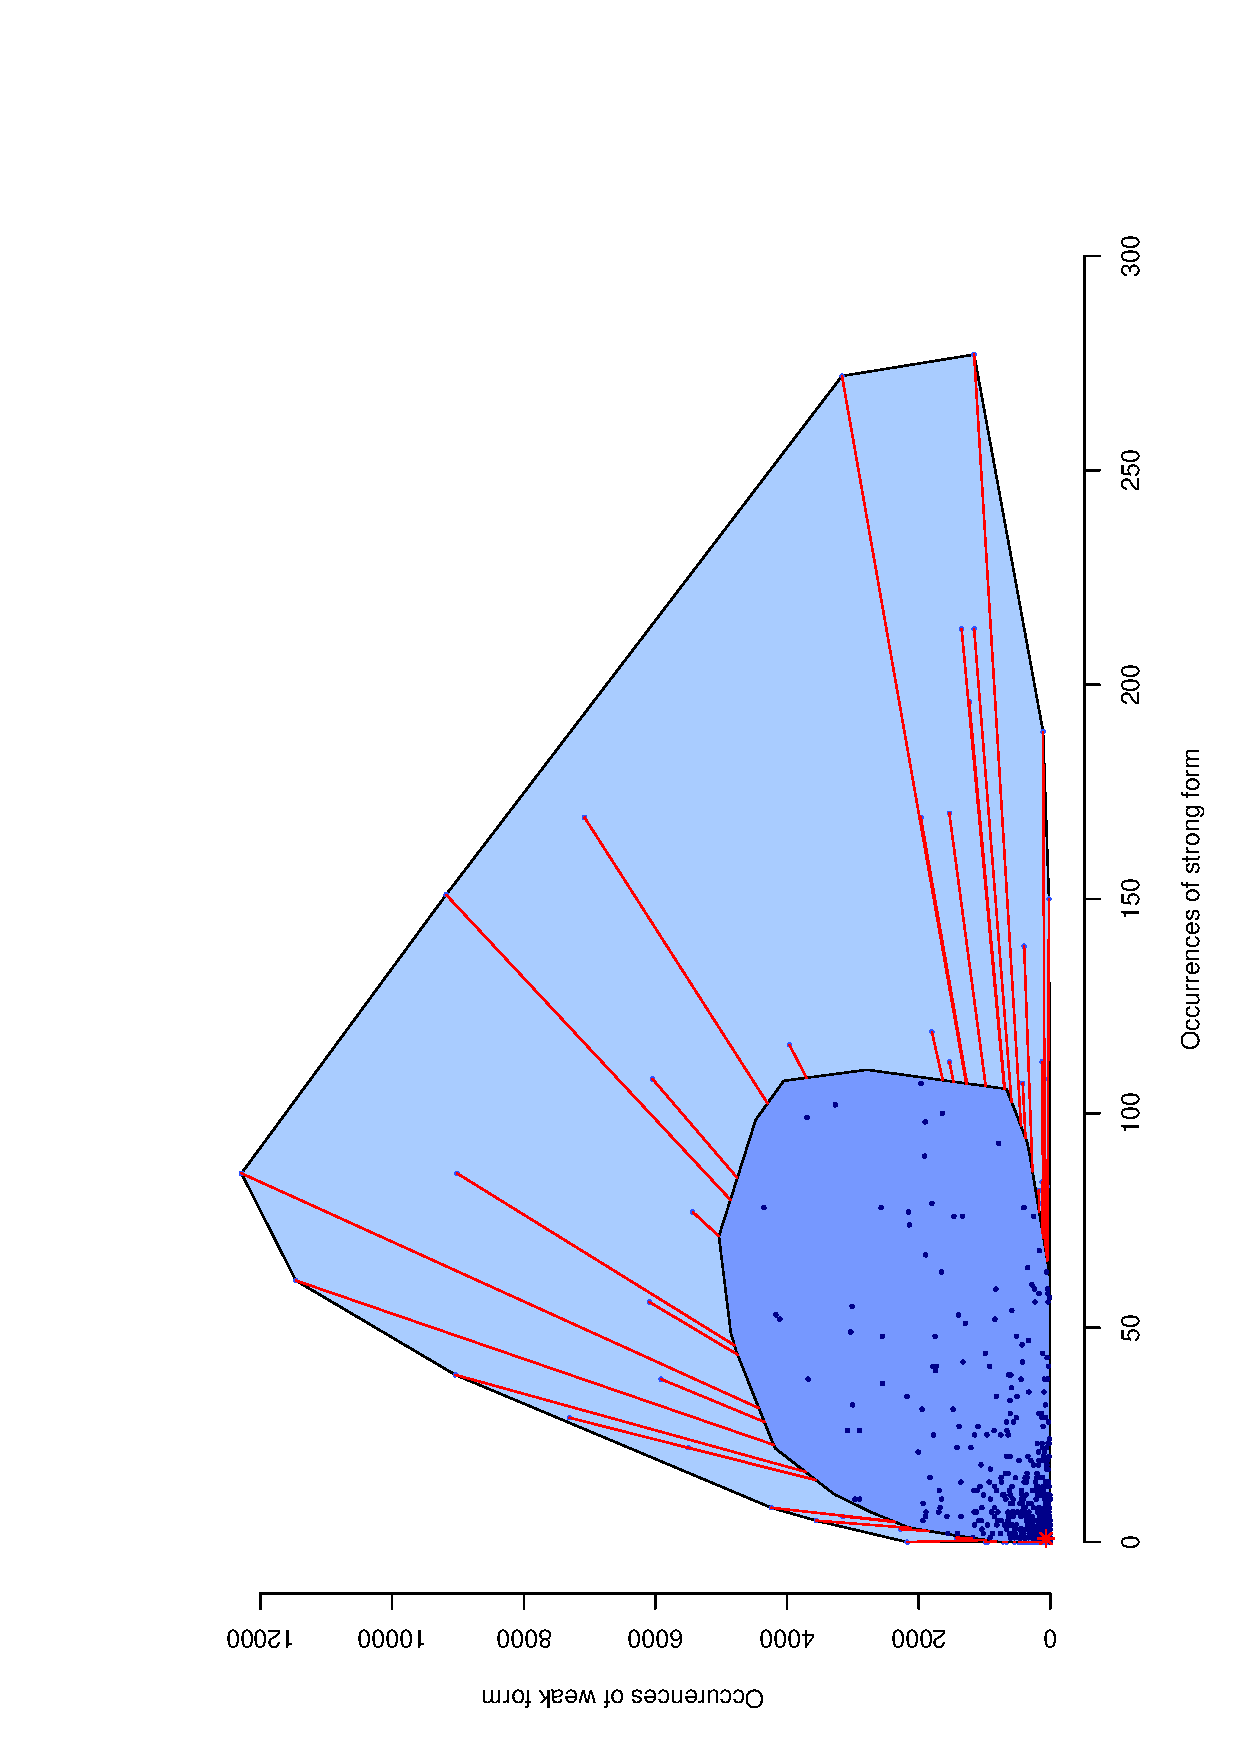
\includegraphics[height=0.95\textheight,angle=270]{bag}
\end{frame}

\begin{frame}
	{Köpckes (1995) Prototypen}
	\centering
	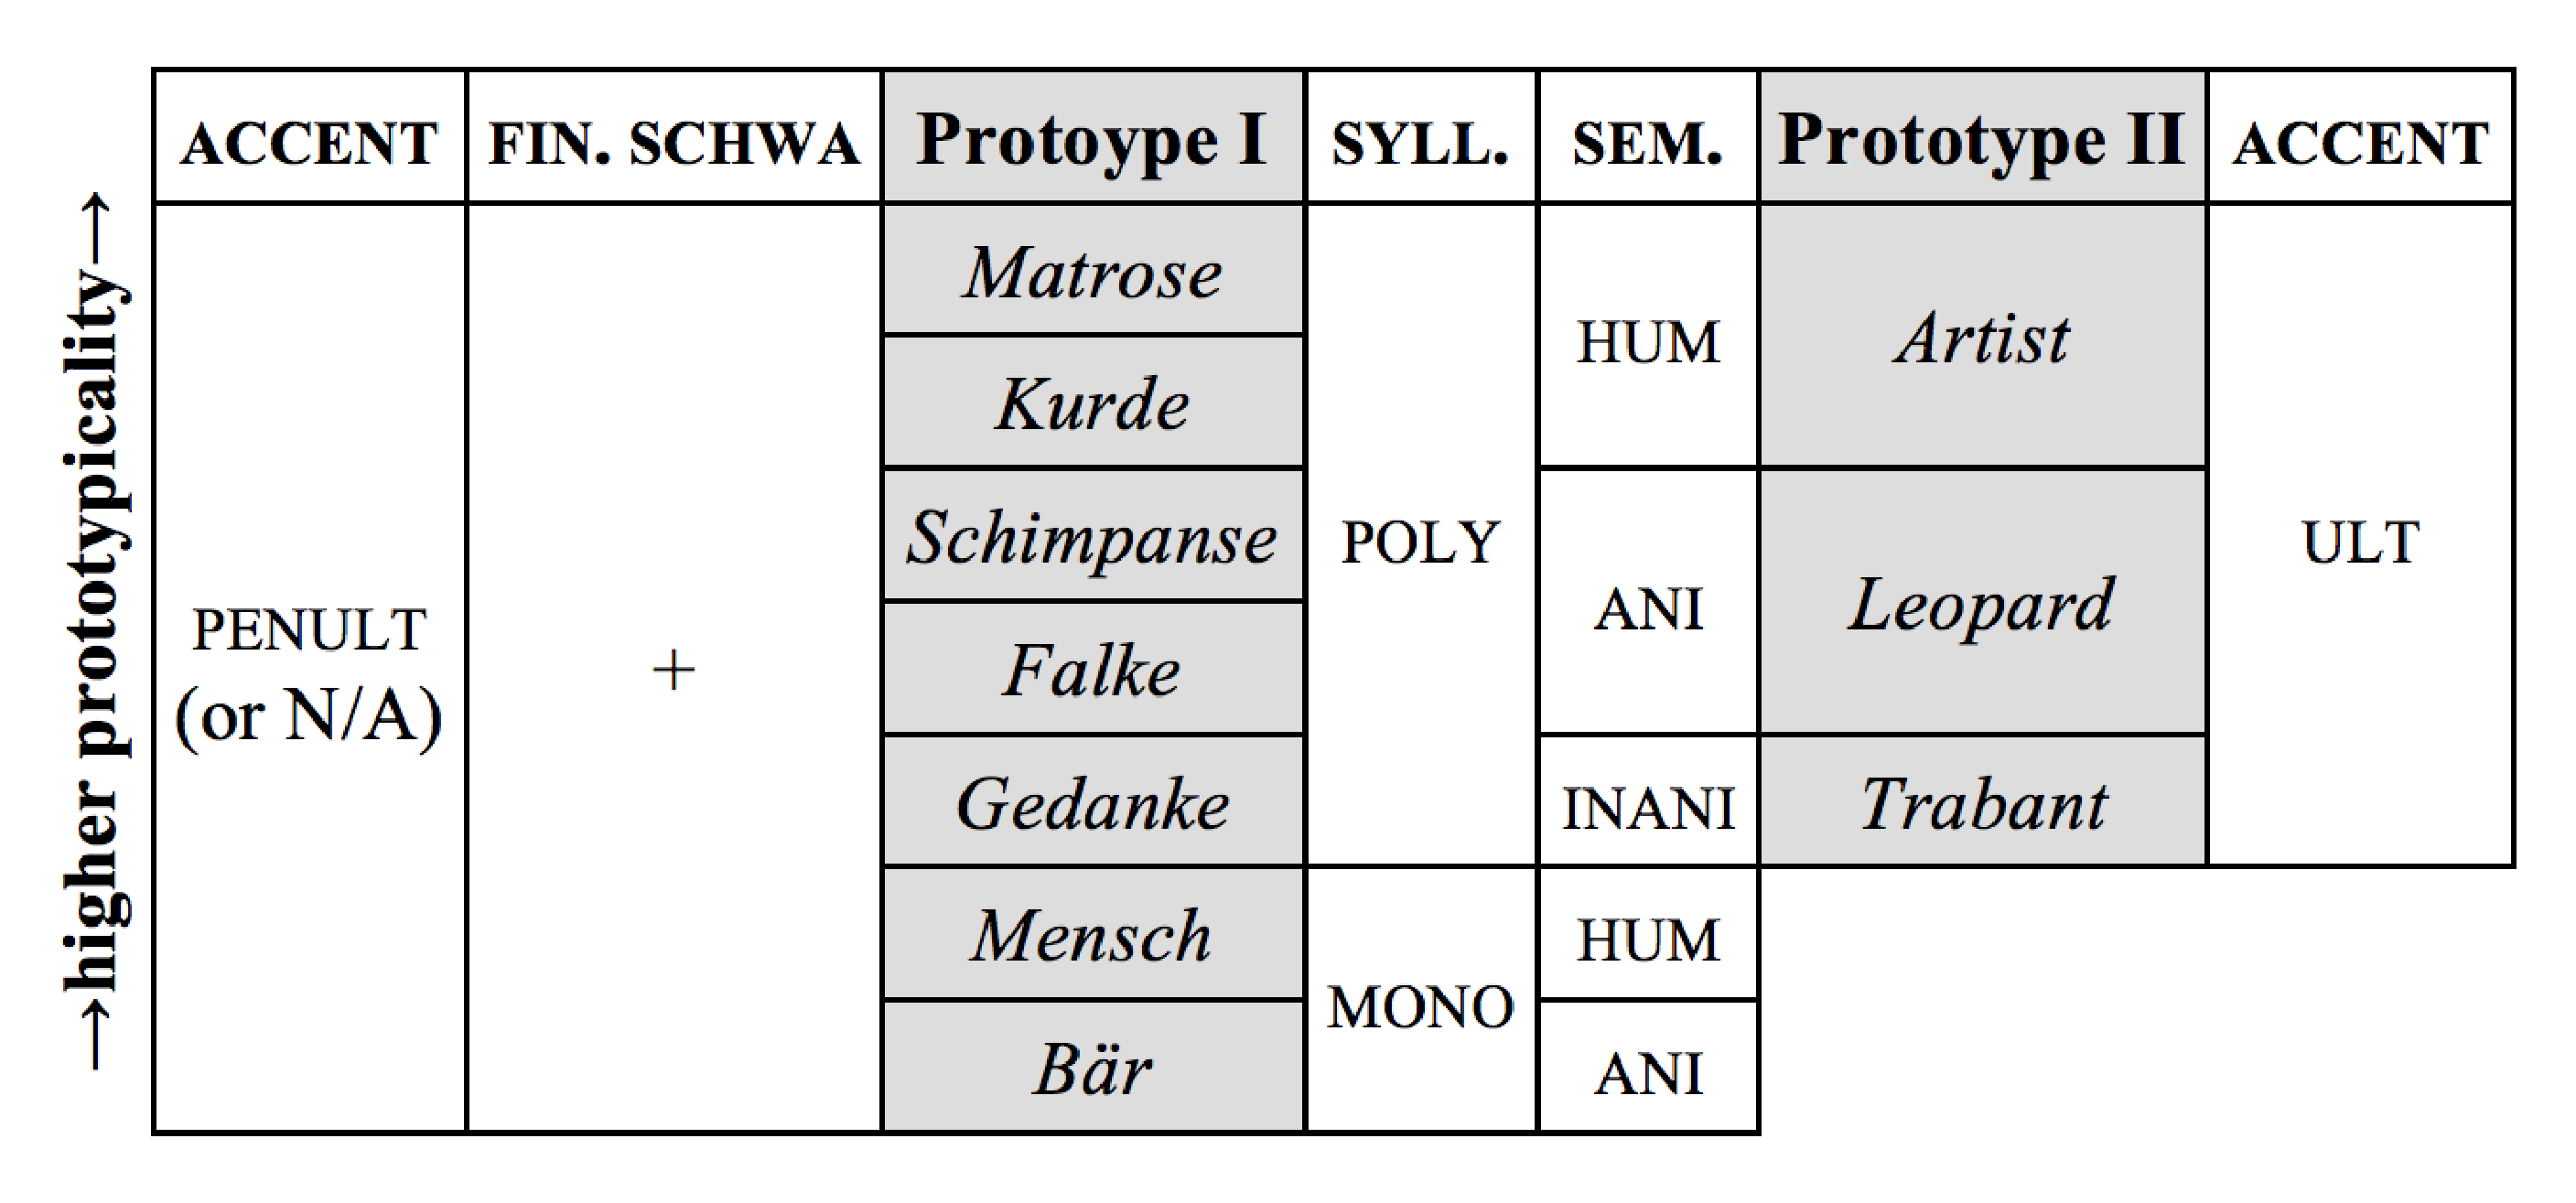
\includegraphics[height=0.6\textheight]{koepcke}
\end{frame}

\begin{frame}
	{... kontrollieren die Alternationsstärke!}
	\centering
	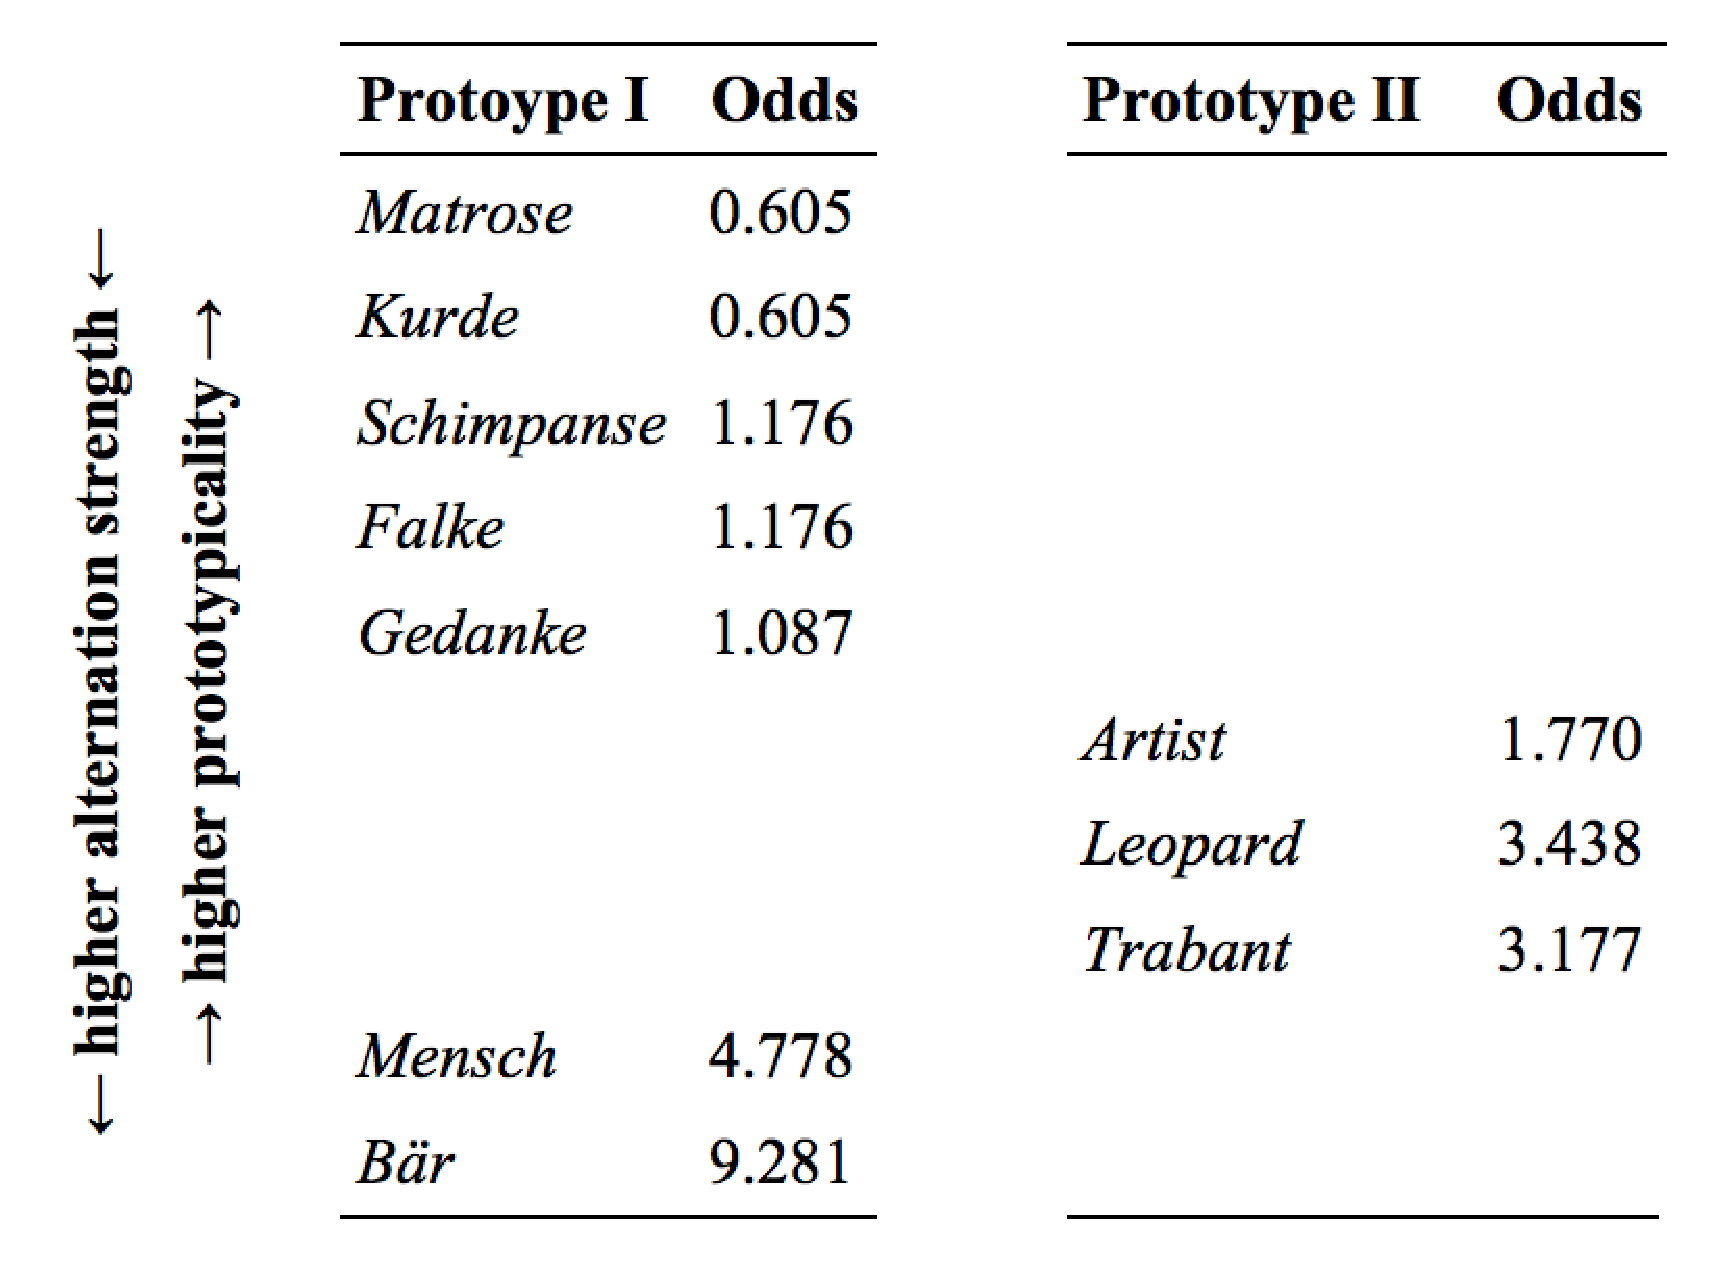
\includegraphics[height=0.6\textheight]{schaefer}\\
	\vspace{0.5cm}
	summierte Chancenverhältnisse für die (Sub-)Prototypen\\
	die Wörter sind nur Beispiele!
\end{frame}

